\chapter{Tecnologias}
Nesse capítulo serão citadas a arquitetura do nosso projeto com ilustrações demonstrando de forma mais lúdica, as possíveis integrações que nossa aplicação terá com sistemas externos.

\section{Arquitetura}
Para o desenvolvimento do projeto, e tendo em vista que será construída uma aplicação web de página única, utilizaremos de ferramentas que cerceiam o ecossistema de \textit{Single Page Applications}. Para isso, teremos a divisão do projeto em \textit{front-end} e \textit{back-end} de modo que eles se comuniquem via protocolo HTTP com requisições e respostas no formato JSON. Para o desenvolvimento do \textit{front-end} utilizaremos Typescript por meio da biblioteca React; o \textit{back-end} será desenvolvido utilizando Java com o micro \textit{framework} Spring Boot. Um módulo de apoio no lado do servidor poderá ser possível, e para ele utilizaremos Python. 

Em relação ao deploy das aplicações, o \textit{front-end} será hospedado na plataforma Vercel, que é primariamente voltada para Javascript, proporcionando uma melhor agilidade de desenvolvimento, enquanto o \textit{back-end} será hospedado no Heroku, que é uma plataforma como serviço de fácil manuseio e que nos permitirá ter um maior foco no desenvolvimento do projeto. Através do Heroku podemos também fazer a utilização do banco de dados PostgreSQL por meio do serviço de apoio Heroku Postgres.

Ademais, se for necessário o armazenamento de objetos como arquivos ou imagens, utilizaremos a plataforma Cloudinary principalmente por sua fácil integração com a linguagem de programação Java através de bibliotecas.


\subsection{Diagramas de arquitetura}
Os diagramas \autoref{fig_arq_app}, \autoref{fig_arq_tec} e \autoref{fig_arq_negocio} ilustram de modo geral a arquitetura pensada para a solução proposta, utilizando das tecnologias já citadas.

\section{Integrações}
Nessa seção serão citadas as possíveis integrações que nossa aplicação terá, que foram decididas baseadas em outras aplicações do mercado.

\subsection{Login com o Google e LinkedIn}
Pensando na experiência de usuário, nossa aplicação terá a opção do estudante se logar através do \ac{sso} dessas empresas. Dessa forma, não será necessário digitar a senha toda vez que o usuário for usar nosso \emph{website}, precisando apenas clicar um botão e fazer o login em uma dessas alternativas.

\subsection{Entrar em contato via \emph{Whatsapp}}
Nossa aplicação terá, também, uma forma da empresa contatar o estudante via Whatsapp. Essa integração será feita via \ac{api} disponibilizada pela própria empresa que mantém o aplicativo (Meta). Dessa forma, com apenas um clique, será possível enviar uma mensagem diretamente ao estudante.

\begin{figure}[htb]
	\centering
	\caption{\label{fig_arq_app}Arquitetura de Aplicação}
	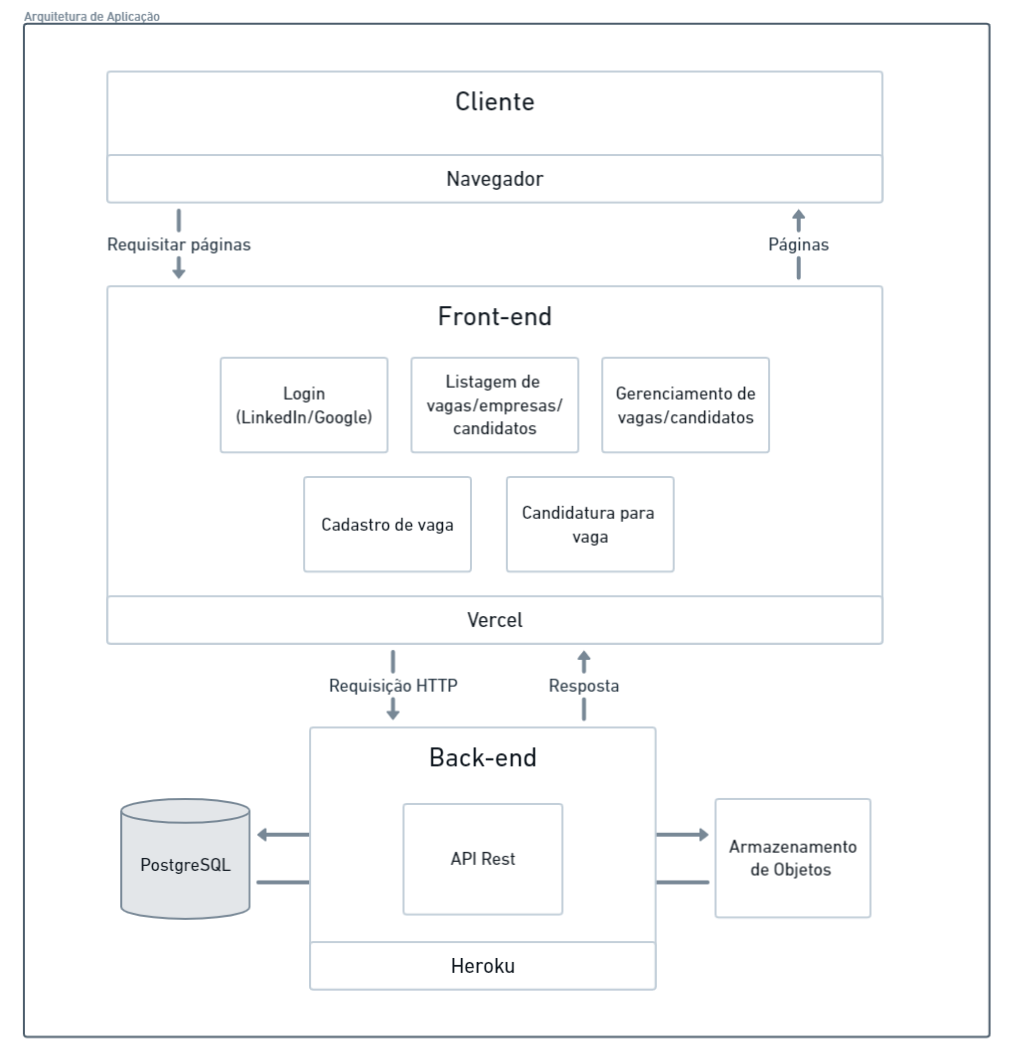
\includegraphics[width=0.95\textwidth]{imagens/arq-proj-arq-app.png}
	\fonte{Produzido pelos autores utilizando a ferramenta \textit{Whimscal}}
\end{figure}

\begin{figure}[htb]
	\centering
	\caption{\label{fig_arq_tec}Arquitetura Tecnológica}
	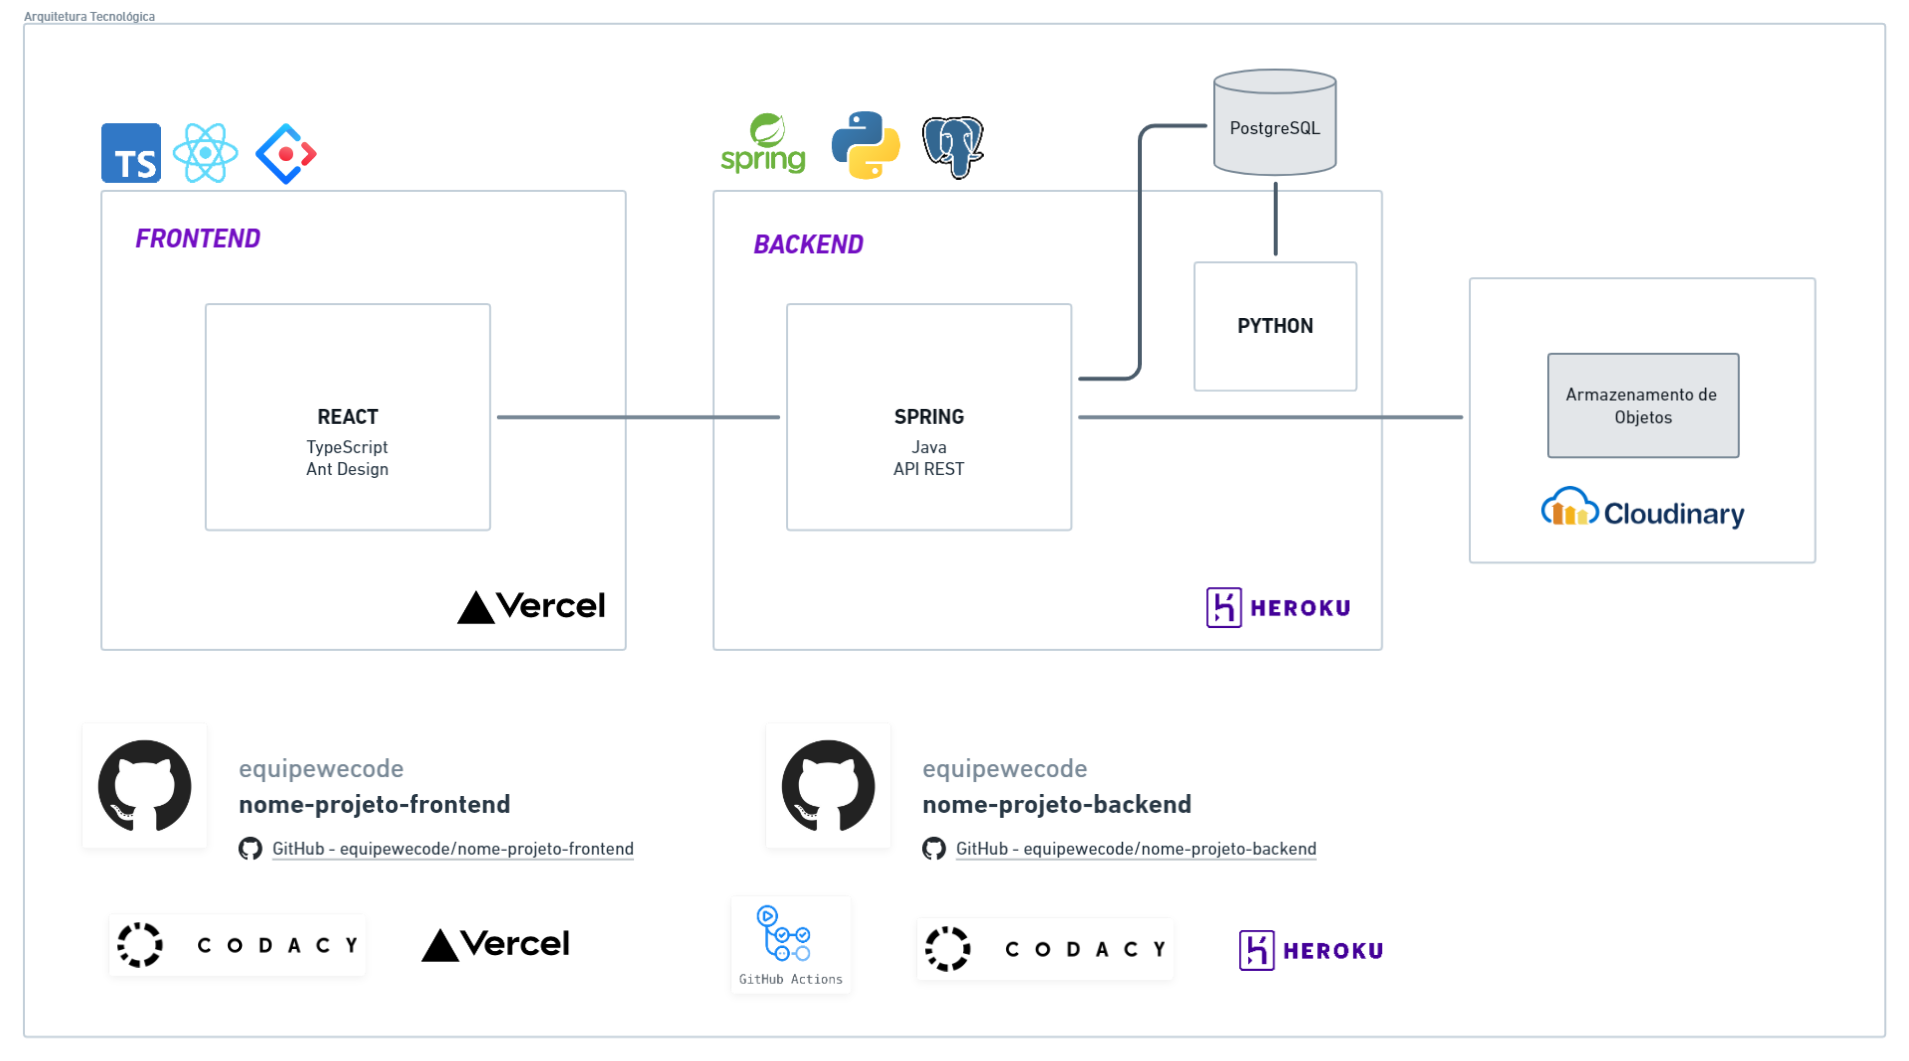
\includegraphics[width=0.95\textwidth]{imagens/arq-proj-arq-tec.png}
	\fonte{Produzido pelos autores utilizando a ferramenta \textit{Whimscal}}
\end{figure}

\begin{figure}[htb]
	\centering
	\caption{\label{fig_arq_negocio}Arquitetura de Negócios}
	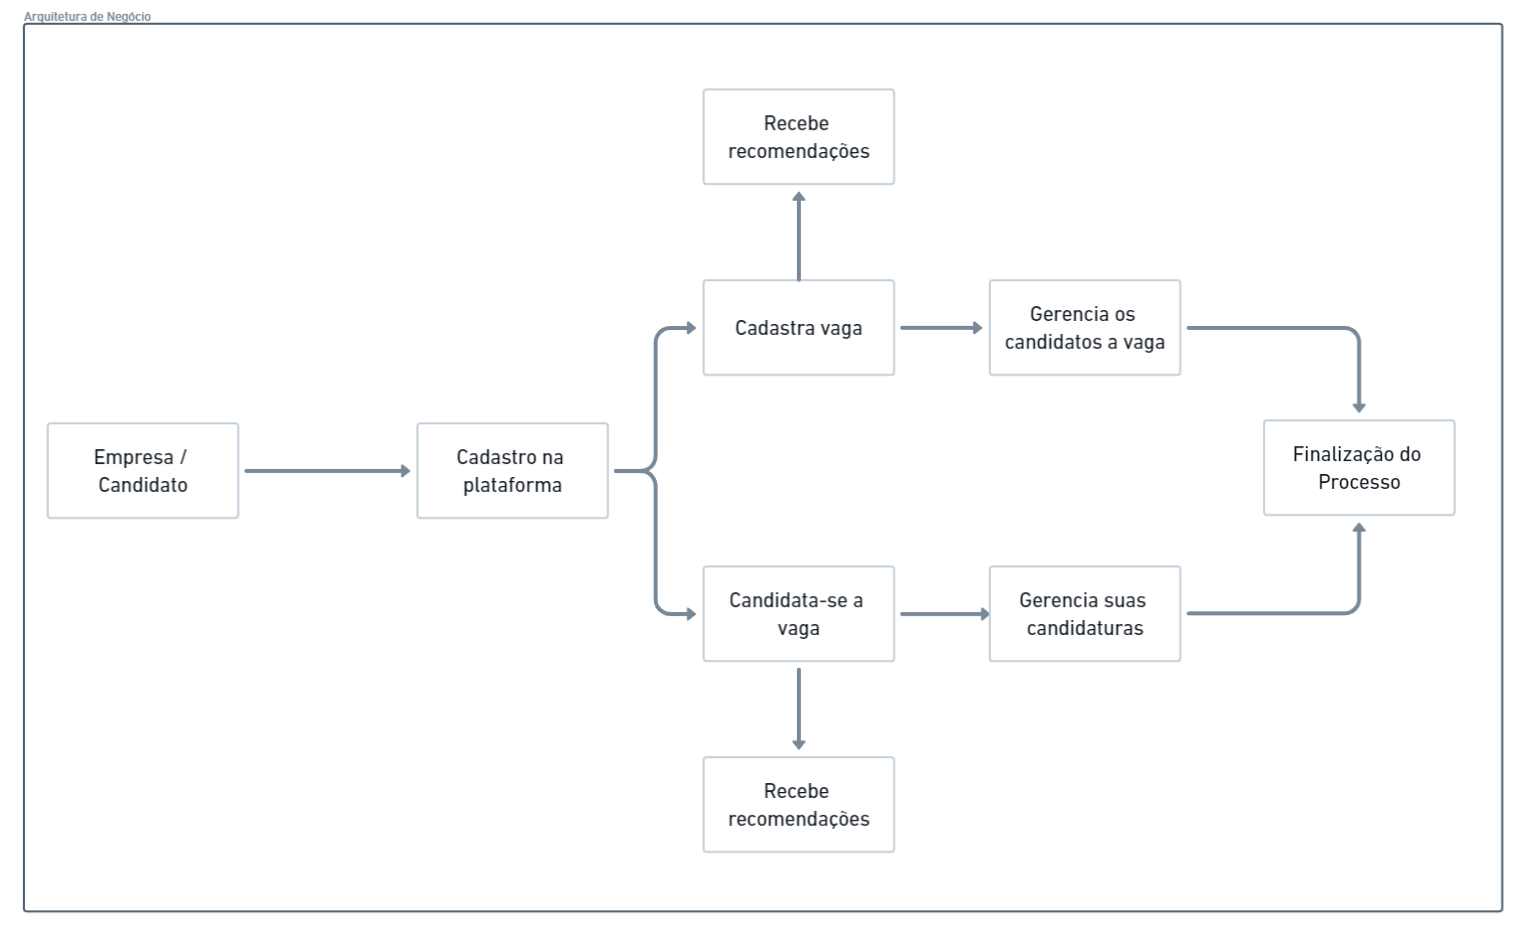
\includegraphics[width=0.95\textwidth]{imagens/arq-proj-arq-negocio.png}
	\fonte{Produzido pelos autores utilizando a ferramenta \textit{Whimscal}}
\end{figure}